% Untangling Federal Jurisdiction
% Part 1 of 3

% All content comes from Stephen Pratt. I have no idea if he approves of this effort or not.

\documentclass[xcolor=usenames,dvipsnames]{beamer}
\usetheme{Madrid}
%\usetheme{Goettingen}
%\usefonttheme{serif}
%\usefonttheme{structuresmallcapsserif}
% \usepackage[font=small,labelfont=bf]{caption}
\usefonttheme{professionalfonts}
\usepackage{xcolor}
\usepackage{rotating}
\usepackage{multirow}
\usepackage{soul}
\usepackage[overlay,absolute]{textpos}

\setbeamerfont{section title}{parent=title}
\setbeamercolor{section title}{parent=titlelike}
\defbeamertemplate*{my section page}{default}[1][]
{
    \centering
    \begin{beamercolorbox}[sep=8pt,center,#1]{section title}
        \usebeamerfont{section title}\insertsection\par
    \end{beamercolorbox}
}

\setbeamertemplate{navigation symbols}{}
\newcommand*{\mysectionpage}{\usebeamertemplate*{my section page}}

\def\Put(#1,#2)#3{\leavevmode\makebox(0,0){\put(#1,#2){#3}}}

\setbeamertemplate{footline}{}

\newenvironment<>{varblock}[2][\textwidth]{
    \begin{center}
        \begin{minipage}{#1}
            \setlength{\textwidth}{#1}
            \begin{actionenv}#3
                \def\insertblocktitle{#2}
                \par
                \usebeamertemplate{block begin}}
            {\par
                \usebeamertemplate{block end}
            \end{actionenv}
        \end{minipage}
    \end{center}
}

\setbeamertemplate{blocks}[default]
\addtobeamertemplate{block begin}{\pgfsetfillopacity{0.92}}{\pgfsetfillopacity{1}}
\newenvironment<>{quotepage}[3]{%
    \begin{frame}[t]%{#1}
        \centering
        %\begin{textblock}{100}[0.2,0](50,11)
            \includegraphics[height=\textheight,width=\textwidth,keepaspectratio]{#2} \\
        %\end{textblock}
        \begin{textblock}{70}[0,1](5,96)
            \begin{varblock}[0.9\paperwidth]{}%[shadow=false,rounded=true]{box2}
            %\colorbox{SeaGreen}{%
            %    \begin{minipage}[b]{0.95\paperwidth}
                    %\pgfsetfillopacity{0.35}
                    \begin{centering}
                    #3
                    % XXX Make this work correctly
                    \ifthenelse{\empty {#3} {}}{ \\ is there something here }{}
                    \end{centering}
                    \vspace{3pt}
                    \begin{minipage}[b]{\textwidth}
                    \hfill \small{#1}
                    \if{#1} \\ \fi
                    \end{minipage}
            %    \end{minipage}
            %}
            \end{varblock}
        \end{textblock}
        %\begin{textblock}
        % XXX Include credits (arg #1) here
        %\end{textblock}
}{%
    \end{frame}
}

\DeclareGraphicsExtensions{.pdf,.png,.jpg}

\setlength{\TPHorizModule}{0.01\paperwidth}
\setlength{\TPVertModule}{0.01\paperheight}
\textblockorigin{0mm}{0mm} % start everything near the top-left corner

\newcommand{\myquote}[3]{%
    \begin{quotepage}{#1}{#2}{#3}
    \end{quotepage}
}

\begin{document}

\title[Untangling Federal Jurisdiction]{Untangling Federal Jurisdiction Within a State}
\author{Stephen Pratt}

\section{A Recurrence to First Principles}

\myquote{Benjamin Franklin}{img/ben-franklin.png}{``A frequent recurrence to \emph{fundamental principles}\ldots is absolutely necessary to preserve the blessings of liberty and keep a government free.''}
%\begin{frame}{Fundamental Principles}
%    \begin{columns}[onlytextwidth]
%        \column{0.5\textwidth}
%            \centering
%            \includegraphics[width=0.75\textwidth]{img/ben-franklin.png} \\
%            Ben Franklin \\
%
%        \column{0.5\textwidth}
%            ``A frequent recurrence to \emph{fundamental principles}\ldots is absolutely necessary to preserve the blessings of liberty and keep a government free.''
%    \end{columns}
%\end{frame}

\begin{frame}{Fundamental Principles}
    \begin{columns}[onlytextwidth]
        \column{0.5\textwidth}
            \centering
            \includegraphics[width=0.75\textwidth]{img/patrick-henry.png} \\
            Patrick Henry \\

        \column{0.5\textwidth}
            ``No free government, or the blessing of liberty, can be preserved to any people but\ldots by a frequent recurrence to \emph{fundamental principles}.
    \end{columns}
\end{frame}

\begin{frame}{Fletcher vs. Peck, 10 U.S. 87}
    \centering
    \includegraphics[width=0.75\textwidth]{img/supreme-court-1810.png} \\
    Supreme Court, 1810 \\
\end{frame}

\begin{frame}{Fletcher vs. Peck, 10 U.S. 87}
    \begin{columns}[onlytextwidth]
        \column{0.5\textwidth}
            \centering
            \includegraphics[width=0.75\textwidth]{img/supreme-court-1810.png} \\
            Supreme Court, 1810 \\

        \column{0.5\textwidth}
            ``The security of a people against the misconduct of their rulers,
            must lie in the frequent recurrence to \emph{first principles}, and
            the imposition of adequate constitutional restrictions.''
    \end{columns}
\end{frame}

\begin{frame}
    \begin{columns}[onlytextwidth]
        \column{0.5\textwidth}
            ``The further back you can look, the farther forward you are likely to see.'' \\
            \vspace{20pt} Statehood, p. 19

        \column{0.5\textwidth}
            \centering
            \includegraphics[width=0.75\textwidth]{img/winston-churchill.png} \\
            Winston Churchill \\
    \end{columns}
\end{frame}

\begin{frame}{Two Contending Forces}
    \begin{columns}[onlytextwidth]
        \column{0.5\textwidth}
            \centering
            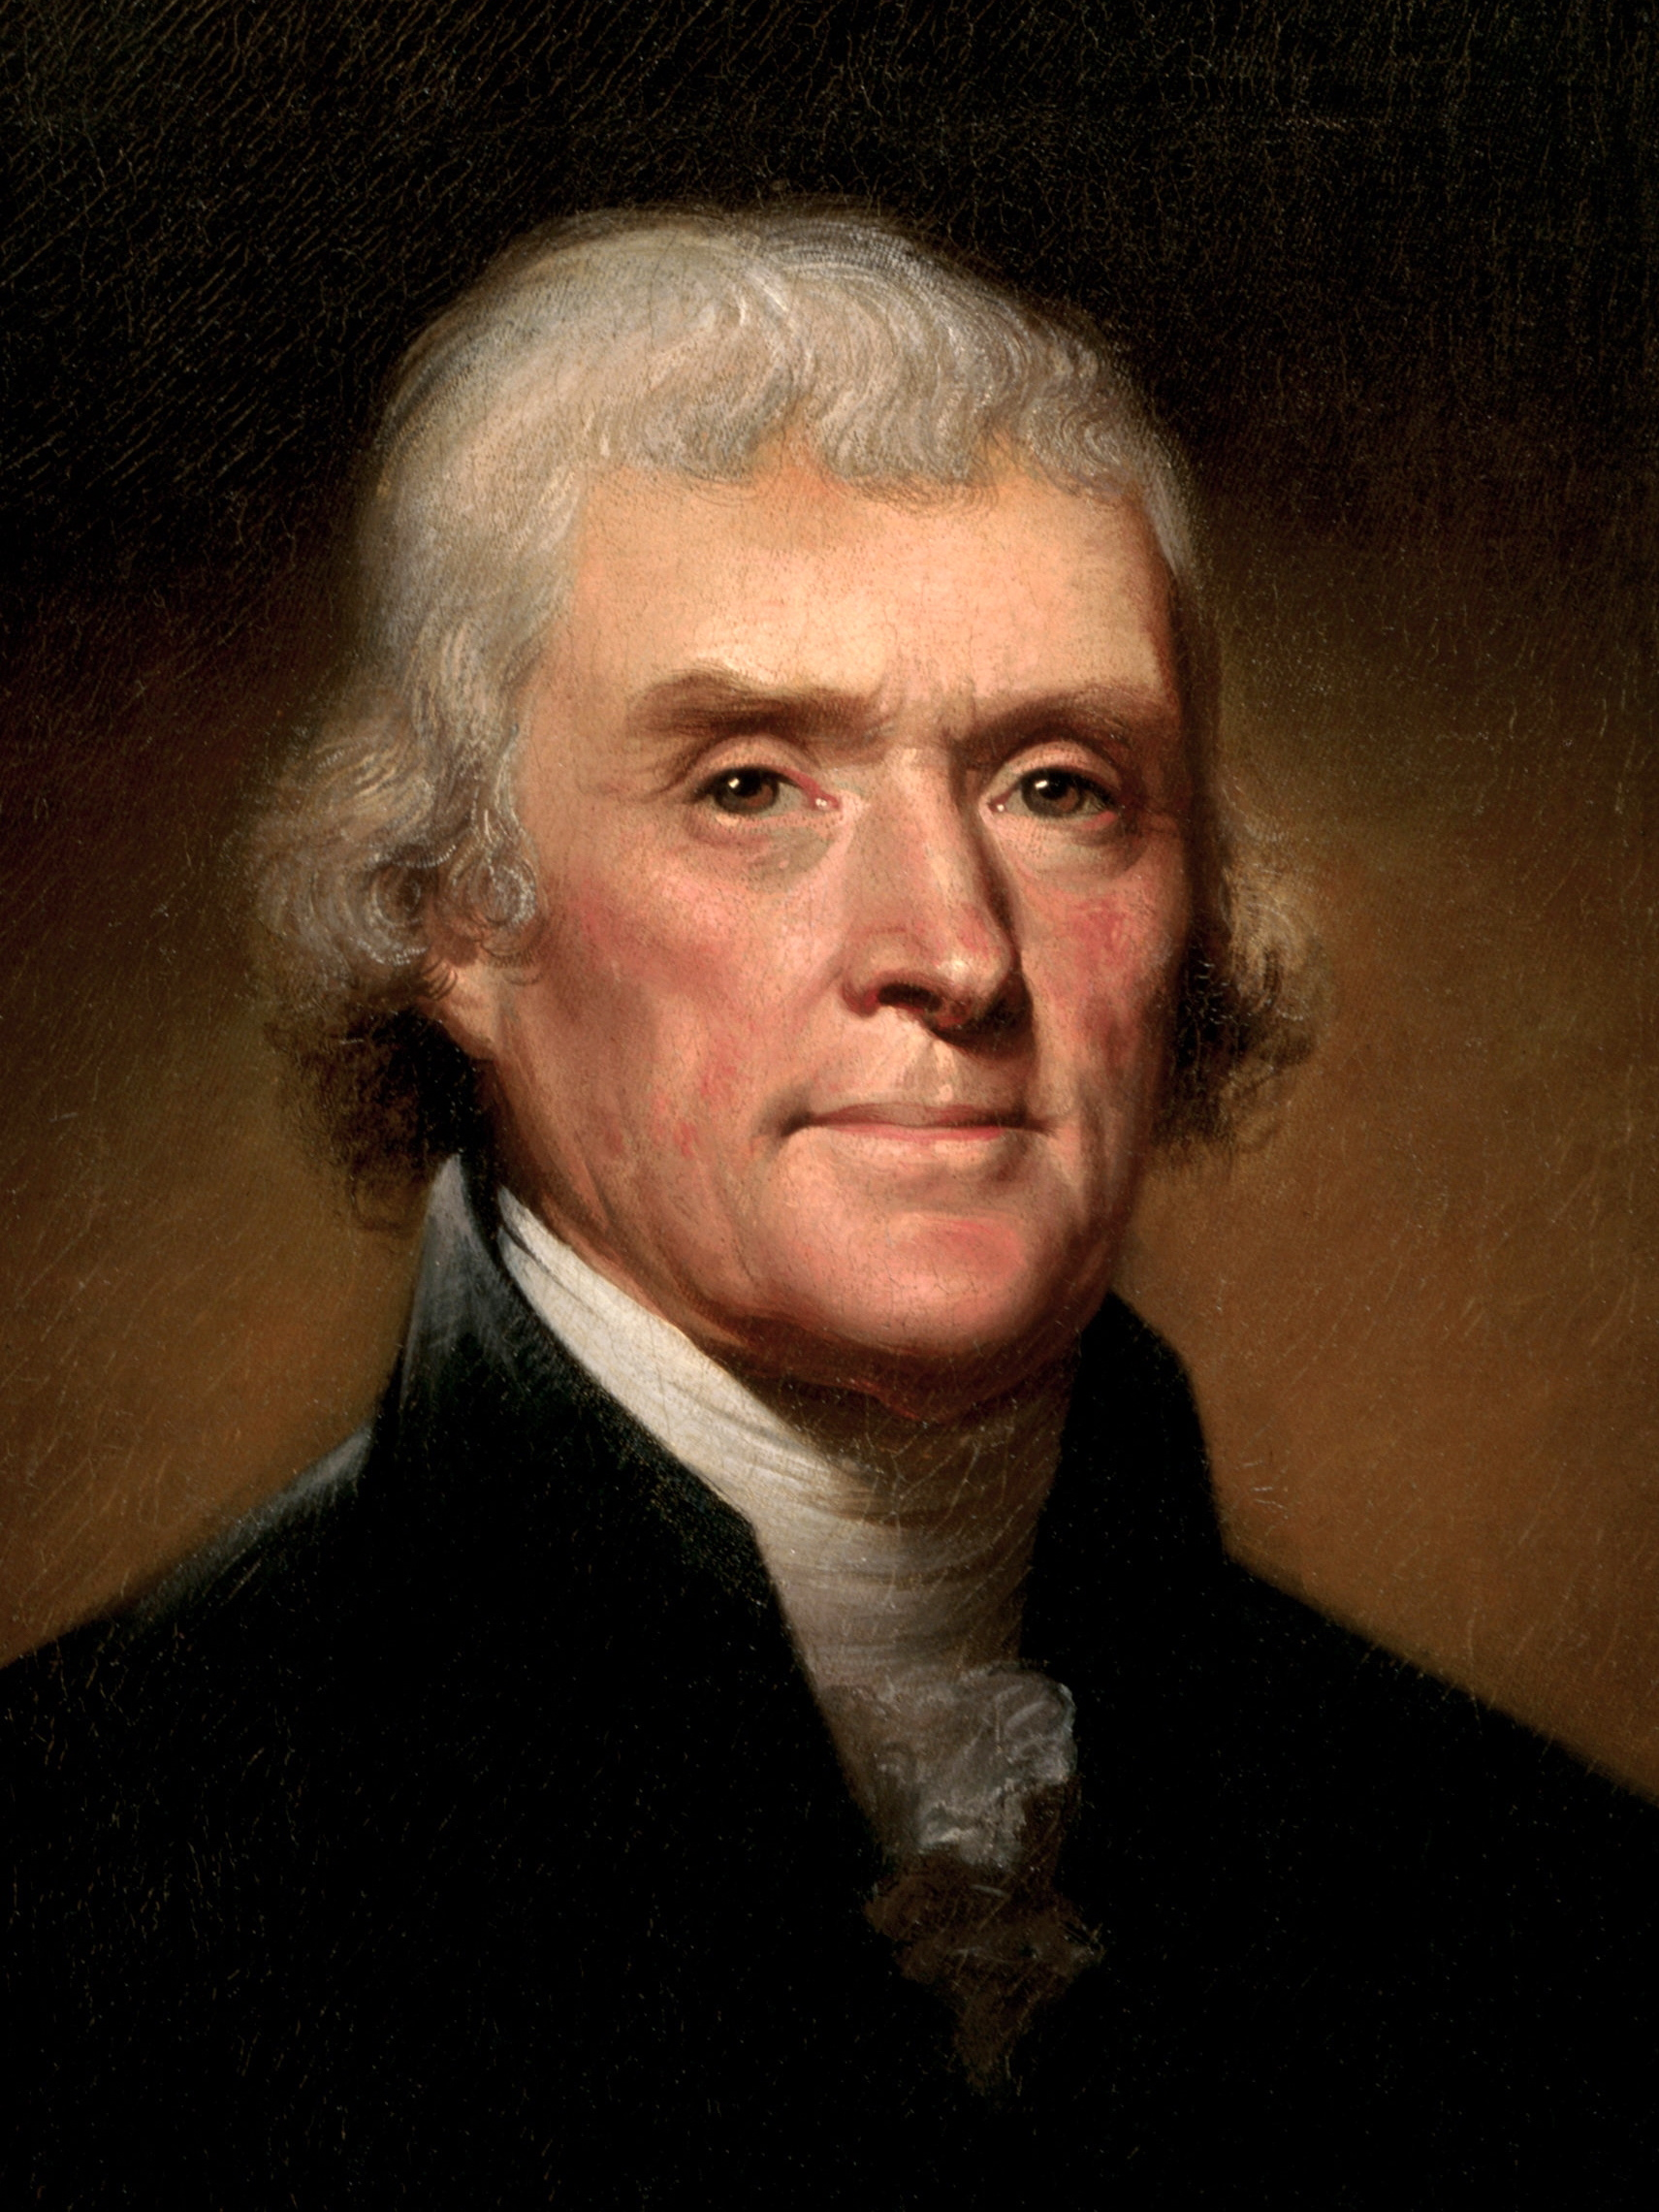
\includegraphics[height=0.75\textheight]{img/jefferson.png} \\
            Thomas Jefferson, 1824

        \column{0.5\textwidth}
            Men by their constitutions are naturally divided into two parties: \\
            \begin{enumerate}
                \item Those who fear and distrust the people, and wish to draw all powers from them into the hands of the higher classes.
                \item Those who identify themselves with the people, [and] have confidence in them.
            \end{enumerate}
    \end{columns}
\end{frame}

\begin{frame}{Roman Civil Law, 9 A. D.}
    \centering
    \includegraphics[width=0.75\textwidth]{img/europe-map.png} \\
    \only<1>{Roman Law \\}
%    \only<2>{Civil Law \\}
%    \only<3>{Roman Civil Law \\}
\end{frame}

\begin{frame}{Roman Law}
    \begin{columns}[onlytextwidth]
        \column{0.5\textwidth}
            \centering
            \includegraphics[height=0.55\textheight]{img/fasces-copy.jpg} \\
            Fasces \\

        \column{0.5\textwidth}
            \begin{itemize}
                \item All powerful central government
                \item National sovereignty
                \item Tax and control everything
                \item Watchdog everyone's business
                \item Promise prosperity and greatness
                \item Fight wars anywhere on earth
                \pause
                \item \emph{Do whatever is necessary. No exceptions. No limits\ldots}
            \end{itemize}
    \end{columns}
\end{frame}

\begin{frame}
    \centering
    \includegraphics[width=0.95\textwidth]{img/teutoburg.png} \\
    Battle of Teutoburg Forest, 9 A. D. \\
        Arminius of the Cherusci, Publius Quinctilius Varus \\
%    \only<2>{``We will rule our own territory!'' \\ }
\end{frame}

\begin{frame}
    \centering
    \includegraphics[width=0.95\textwidth]{img/teutoberg.jpg} \\
    Battle of Teutoburg Forest, 9 A. D. \\
        Arminius of the Cherusci, Publius Quinctilius Varus \\
%    \only<2>{``We will rule our own territory!'' \\ }
\end{frame}

\begin{frame}
    \centering
    \includegraphics[width=0.95\textwidth]{img/Varus01.jpg} \\
    Battle of Teutoburg Forest, 9 A. D. \\
        Arminius of the Cherusci, Publius Quinctilius Varus \\
%    \only<2>{``We will rule our own territory!'' \\ }
\end{frame}

\begin{frame}
    \centering
    \includegraphics[height=0.8\textheight]{img/teut2.jpg} \\
    Battle of Teutoburg Forest, 9 A. D. \\
        Arminius of the Cherusci, Publius Quinctilius Varus \\
%    \only<2>{``We will rule our own territory!'' \\ }
\end{frame}

\begin{frame}
    \centering
    \includegraphics[height=0.8\textheight]{img/teut3.jpg} \\
    Battle of Teutoburg Forest, 9 A. D. \\
        Arminius of the Cherusci, Publius Quinctilius Varus \\
%    \only<2>{``We will rule our own territory!'' \\ }
\end{frame}

\begin{frame}
    \centering
    \includegraphics[width=0.95\textwidth]{img/teut4.png} \\
    Battle of Teutoburg Forest, 9 A. D. \\
        Arminius of the Cherusci, Publius Quinctilius Varus \\
%    \only<2>{``We will rule our own territory!'' \\ }
\end{frame}

\begin{frame}
    \centering
    \includegraphics[width=0.95\textwidth]{img/teut5.png} \\
    Battle of Teutoburg Forest, 9 A. D. \\
        Arminius of the Cherusci, Publius Quinctilius Varus \\
%    \only<2>{``We will rule our own territory!'' \\ }
\end{frame}

\begin{frame}{Anglo-Saxon Common Law}
    \begin{columns}[onlytextwidth]
        \column{0.5\textwidth}
            Germanic brothers who entered England in 450 A. D., bringing with them Anglo-Saxon Common Law, the ``Guardian of Freedom''.

        \column{0.5\textwidth}
            \centering
            \includegraphics[height=0.55\textheight]{img/hengist-horsa.png} \\
            Hengist and Horsa \\
    \end{columns}
\end{frame}

\begin{frame}{Germany, 1875 --- Hermanns Denkmal}
    \centering
    \includegraphics[width=0.75\textwidth]{img/hermans-denkmal.png} \\
\end{frame}

\begin{frame}{Germany, 1875 --- Hermanns Denkmal}
    \centering
    \includegraphics[width=0.75\textwidth]{img/herman2.png} \\
\end{frame}

\begin{frame}
    \begin{columns}[onlytextwidth]
        \column{0.5\textwidth}
            \centering
            \includegraphics[width=0.75\textwidth]{img/herman2.png} \\

        \column{0.5\textwidth}
            Arminius / Herman preserved ``Common Law''
            \pause
            \begin{itemize}
                \item Higher Law
                \pause
                \item Law of Nature
                \pause
                \item Constrast with Roman Law, based on coercion and force
            \end{itemize}
    \end{columns}
\end{frame}

\begin{frame}{Fundamental Principles of Common Law}
    \centering
    \includegraphics[width=0.75\textwidth]{img/schoolroom.png} \\
\end{frame}

\begin{frame}{Preserve Our Principles}
    \centering
    \includegraphics[width=0.75\textwidth]{img/herman3.png} \\
    Rome, go home! \\
\end{frame}

\begin{frame}{Preserve Our Principles}
    \begin{columns}[onlytextwidth]
        \column{0.5\textwidth}
            \centering
            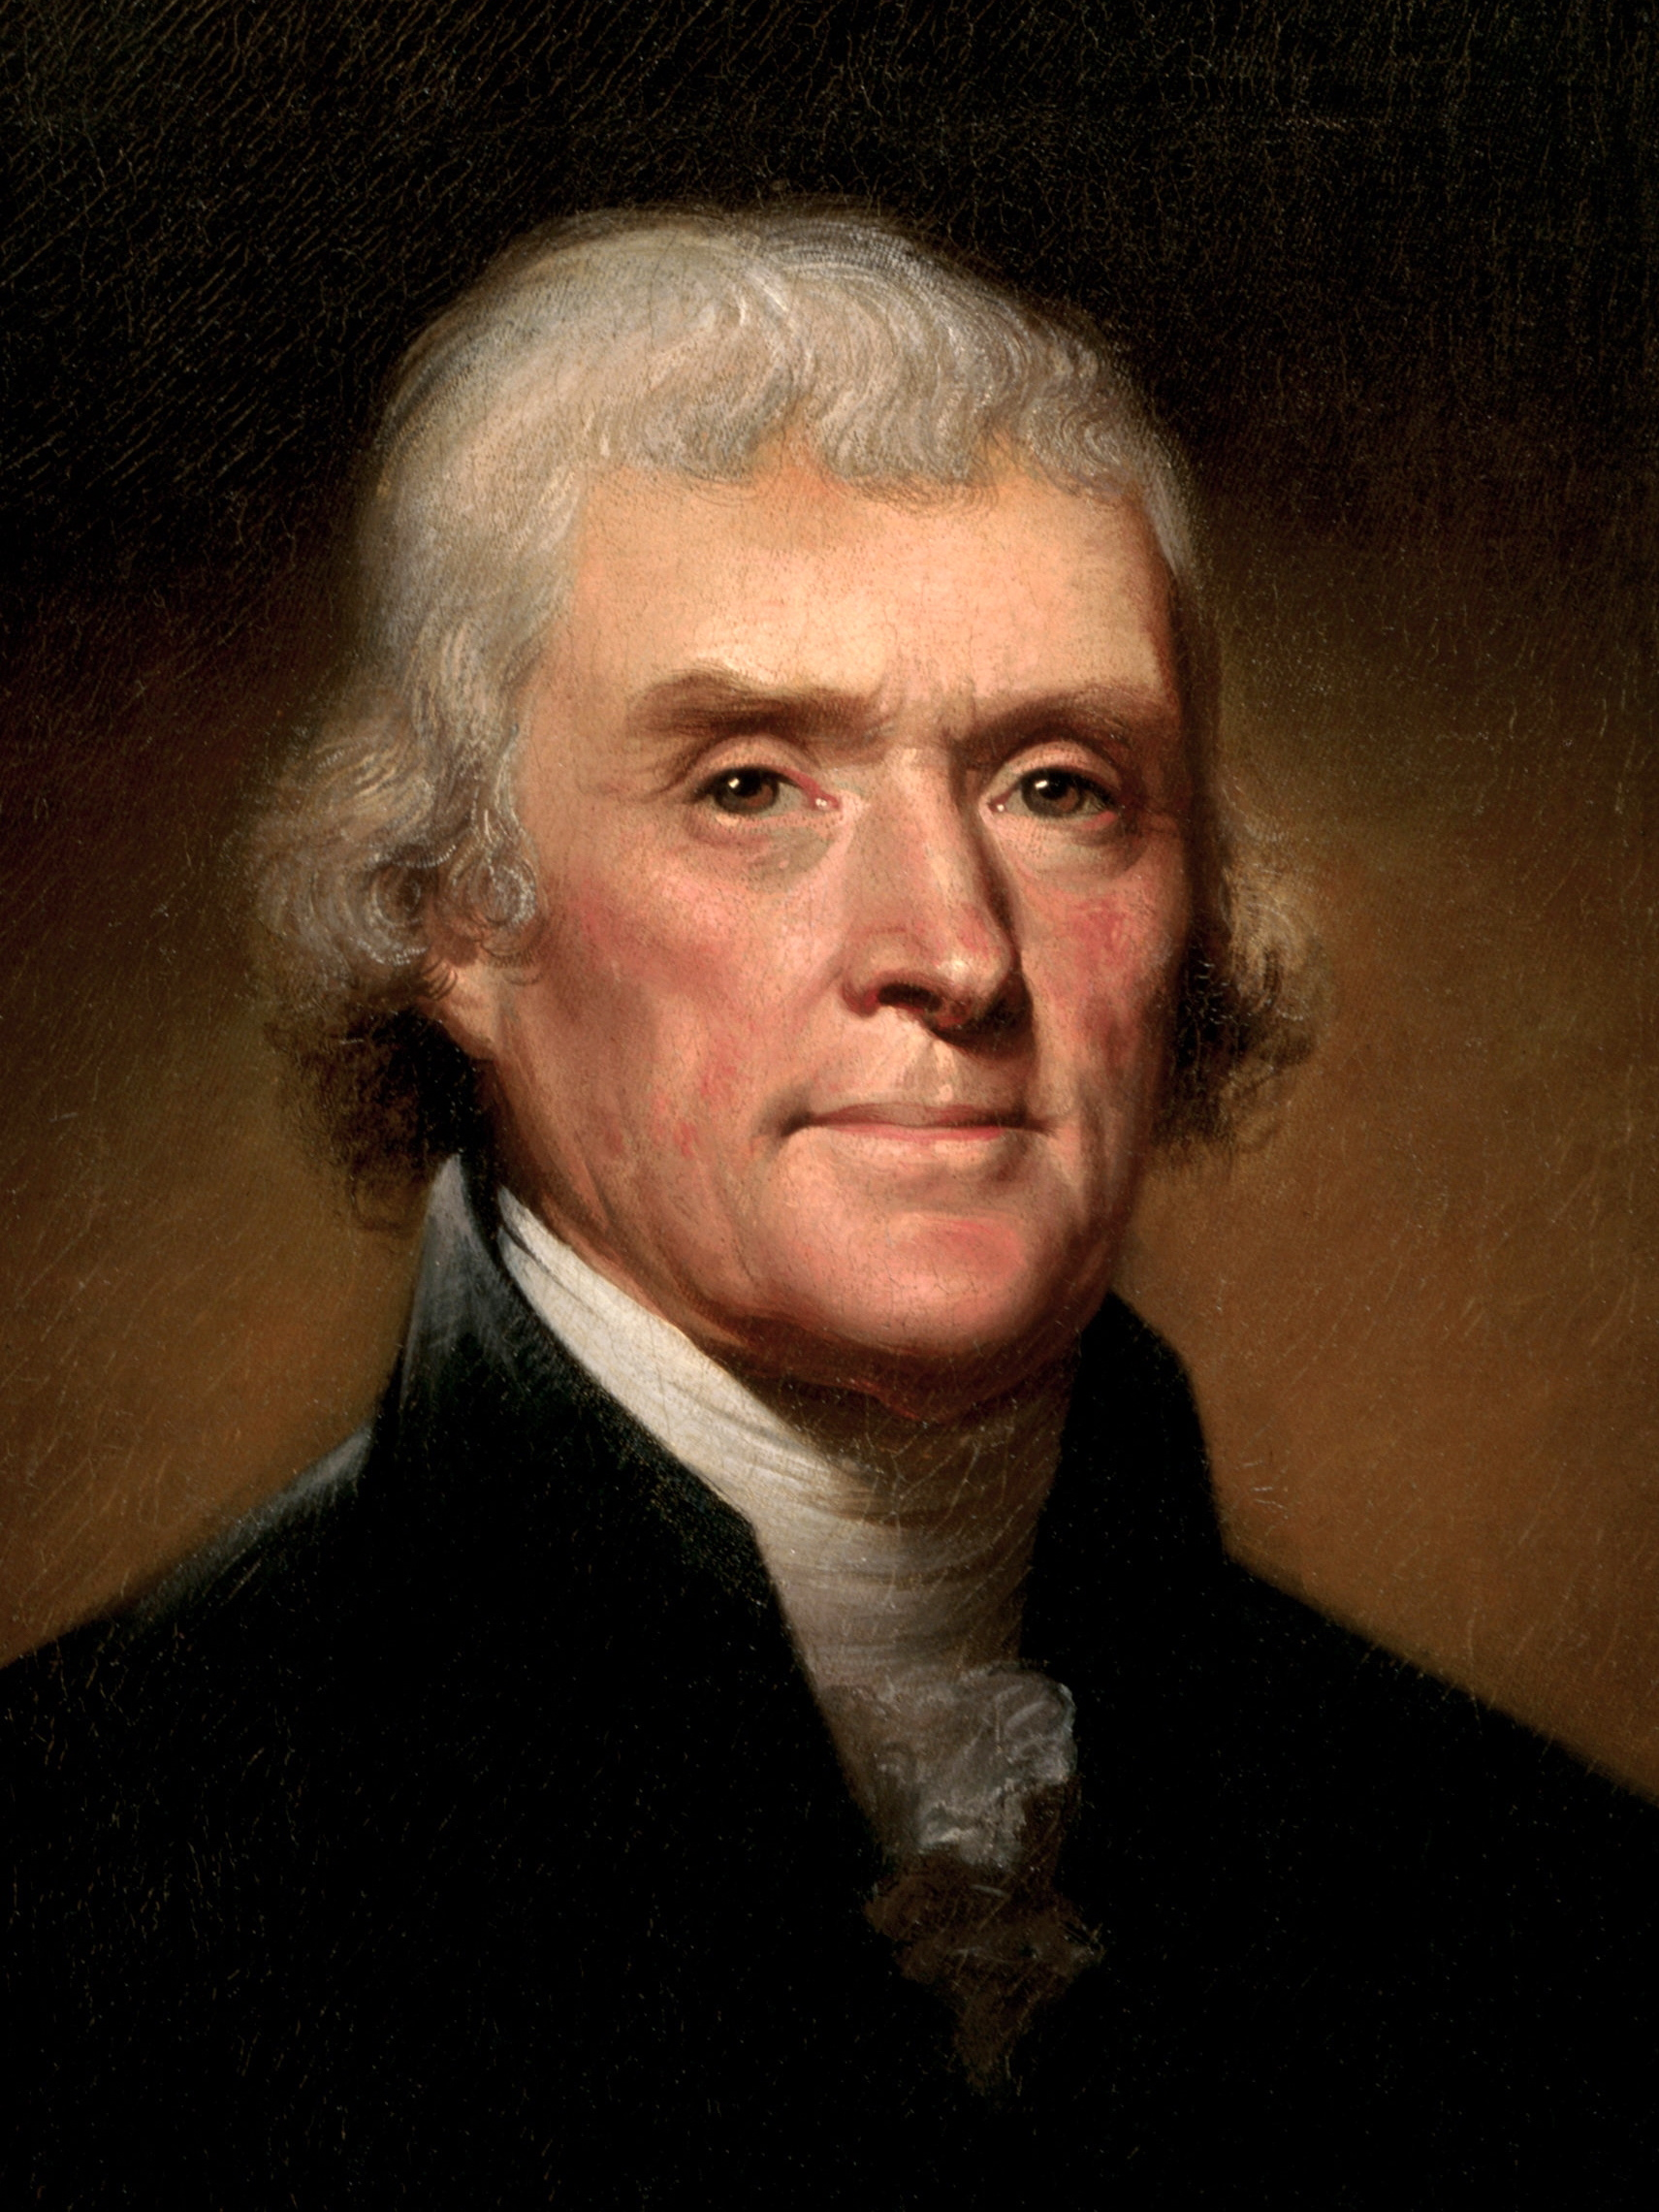
\includegraphics[width=0.75\textwidth]{img/jefferson.png} \\
            Thomas Jefferson \\

        \column{0.5\textwidth}
            Restore the Ancient Principles\ldots
            \begin{itemize}
                \item \ldots of Common Law
                \item \ldots of the Old Testament
            \end{itemize}
    \end{columns}
\end{frame}

\begin{frame}{Government of Ancient Israel}
    \centering
    \includegraphics[width=0.75\textwidth]{img/moses.jpg} \\
    \only<1>{
        And Moses' father-in-law said unto him: Thou shalt teach them ordinances and laws, and shalt show them the way wherein they must walk and the work that they must do.
    }
    \only<2>{ Groups of tens, fifties, hundreds, thousands, to successfully govern three million people \\ }
%    \only<3>{ This became the basis of ``Common'', or ``People's'' Law \\ }
\end{frame}

\begin{frame}{Preserve Our Principles}
    \begin{columns}[onlytextwidth]
        \column{0.5\textwidth}
            \centering
            \includegraphics[width=0.75\textwidth]{img/moses.jpg} \\
            Anglo-Saxon Common Law \color{red}\\

        \column{0.5\textwidth}
            \begin{itemize}
                \item Ten families --- a ``Tithing'', led by a ``tithing man''
                \item Two tithings --- a ``Vil'', led by a ``vil man''
                \item Two vils --- a ``Hundred'', led by a ``hundred man''
                \item Several hundreds --- a ``Shire'', led by a ``shire reef''
            \end{itemize}
    \end{columns}
\end{frame}

\begin{frame}{Roman Law v. Common Law}
    \begin{columns}[onlytextwidth]
        \column{0.5\textwidth}
            \centering
            \includegraphics[height=0.75\textheight]{img/fasces-copy.jpg} \\

        \column{0.5\textwidth}
            \centering
            \includegraphics[height=0.35\textheight]{img/hh-coin.png} \\
            \includegraphics[height=0.35\textheight]{img/israel-coin.png} \\
    \end{columns}
\end{frame}

\begin{frame}{1914}
    \centering
    \includegraphics[width=.9\textwidth]{img/lincoln-memorial.jpg} \\
\end{frame}

\begin{frame}
    \begin{columns}[onlytextwidth]
        \column{0.5\textwidth}
            \centering
            \includegraphics[width=0.75\textwidth]{img/americas-caesar.png} \\

        \column{0.5\textwidth}
            \begin{block}{America's Caesar}
                The Decline and Fall of Republican Government in the United States of America
            \end{block}
    \end{columns}
\end{frame}

\begin{frame}
    \begin{columns}[onlytextwidth]
        \column{0.5\textwidth}
            \centering
            \includegraphics[width=0.75\textwidth]{img/dime-usa-fasces-2.jpg} \\
            1916 - 1945 \\

        \column{0.5\textwidth}
            \centering
            \includegraphics[height=0.55\textheight]{img/fasces-copy.jpg} \\
            Roman Law\\

    \end{columns}
\end{frame}

\begin{frame}
    \centering
    \includegraphics[width=.9\textwidth]{img/obama-fasces.jpg} \\
\end{frame}

\begin{frame}
    \centering
    \includegraphics[height=.8\textheight]{img/fasces/badge_description.jpg} \\
    Los Angeles Police Dept. badge, developed 1939 - 1941 \\
\end{frame}
\begin{frame}
    \centering
    \includegraphics[height=.8\textheight]{img/fasces/coin.jpg} \\
    Italian East Africa Campaign medal, 1936 \\
\end{frame}
\begin{frame}
    \centering
    \includegraphics[width=.9\textwidth]{img/fasces/fake-fasces.jpg} \\
    Catalonia (largely autonomous Spanish province), 2006 \\
\end{frame}
\begin{frame}
    \centering
    \includegraphics[height=.8\textheight]{img/fasces/fasces13.jpg} \\
    Adopted 1877. Text reads ``Union and Consitution''. Colorado's state website claims ``The Roman fasces is the insignia of a republican form of government\ldots The axe symbolizes authority and leadership.'' \\
\end{frame}
\begin{frame}
    \centering
    \includegraphics[height=.8\textheight]{img/fasces/fasces5coin.jpg} \\
\end{frame}
\begin{frame}
    \centering
    \includegraphics[width=.9\textwidth]{img/fasces/fasces_congress.jpg} \\
\end{frame}
\begin{frame}
    \centering
    \includegraphics[width=.9\textwidth]{img/fasces/fasces-stuff.jpg} \\
    Statue by John Quincy Adams Ward, 1882.
\end{frame}
\begin{frame}
    \centering
    \includegraphics[width=.9\textwidth]{img/fasces/ows.jpg} \\
    Federal Hall, New York City \\
\end{frame}
\begin{frame}
    \centering
    \includegraphics[height=.8\textheight]{img/fasces/flag-fasces.jpg} \\
\end{frame}
\begin{frame}
    \centering
    \includegraphics[height=.8\textheight]{img/fasces/french-republic-symbol.png} \\
    National Symbol of France, adopted 1953. This symbol is used to represent France in the U.N. Assembly building. \\
\end{frame}
\begin{frame}
    \centering
    \includegraphics[height=.8\textheight]{img/fasces/houdon-front.jpg} \\
    Statue by Jean-Antoine Houdon, completed 1791. Commissioned by Virgina's legislature, and on display at Colonial Williamsburg. \\
\end{frame}
\begin{frame}
    \centering
    \includegraphics[height=.8\textheight]{img/fasces/italy-fasces-coin.jpg} \\
    Italian 5 lira piece, 1928 \\
\end{frame}
\begin{frame}
    \centering
    \includegraphics[height=.9\textheight]{img/fasces/jfk.jpg} \\
\end{frame}
\begin{frame}
    \centering
    \includegraphics[width=.9\textwidth]{img/fasces/lincoln_fasces.jpg} \\
\end{frame}
\begin{frame}
    \centering
    \includegraphics[width=.9\textwidth]{img/fasces/manhole.JPG} \\
\end{frame}
\begin{frame}
    \centering
    \includegraphics[height=.8\textheight]{img/fasces/mp.jpg} \\
\end{frame}
\begin{frame}
    \centering
    \includegraphics[height=.8\textheight]{img/fasces/tax-court.png} \\
    The Tax Court took on its present form in 1969 \\
\end{frame}
\begin{frame}
    \centering
    \includegraphics[height=.8\textheight]{img/fasces/teut1.jpg} \\
    Detail of frieze in the U.S. Capitol rotunda. The frieze was designed in 1859 and begun in 1877, but wasn't fully complete until 1953. \\
\end{frame}
\begin{frame}
    \centering
    \includegraphics[width=.9\textwidth]{img/fasces/tunnel.jpg} \\
\end{frame}
\begin{frame}
    \centering
    \includegraphics[height=.8\textheight]{img/fasces/washington1.jpg} \\
    By Horatio Greenough, completed in 1840, and now found in the Smithsonian
    museum of American History. The base reads,``Horatio Greenough made this
    image as a great example of freedom, and will not survive without freedom
    itself.''
\end{frame}

\begin{frame}
    \centering
    \includegraphics[width=.9\textwidth]{img/reich-stamp.png} \\
\end{frame}

\begin{frame}{Two Contending Forces}
    \begin{columns}[onlytextwidth]
        \column{0.5\textwidth}
            \begin{varblock}[0.9\textwidth]{}\huge{ \centering Sovereignty of the National Government \\}\end{varblock}

        \column{0.5\textwidth}
            \begin{varblock}[0.9\textwidth]{}\huge{ \centering Sovereignty of the individual States \\}\end{varblock}
    \end{columns}
    \textbf{\huge{ \color{red}
        \Put(155,120){v.}
    }}
\end{frame}

\begin{frame}
    \centering
    \includegraphics[width=.9\textwidth]{img/supremecourtfasces.jpg} \\
    \large{ Front of the Supreme Court building } \\
\end{frame}

\begin{frame}
    \centering
    \includegraphics[height=.85\textheight]{img/fasces_west_supcourt.jpg} \\
    \large{ On November 28, 2008, 172 pounds of this facade fell four stories to land on the steps of the court } \\
\end{frame}

\begin{frame}
    \centering
    \includegraphics[height=.9\textheight]{img/moses_east_supcourt.jpg} \\
    \large{ Rear of the Supreme Court building } \\
\end{frame}

\begin{frame}
    \centering
    \includegraphics[width=.9\textwidth]{img/10-commandments.jpg} \\
\end{frame}

\end{document}
